\documentclass[a4paper, 11pt]{book}
\usepackage[T1]{fontenc}
\usepackage[utf8]{inputenc}
\usepackage[spanish, es-tabla]{babel}
\usepackage{graphicx}
\graphicspath{ {./images/} }
\usepackage{titling}
\usepackage{ragged2e}
\usepackage[hidelinks]{hyperref}
\usepackage[]{titlesec} % Personalización de títulos
\usepackage{titletoc} % Personalización del índice
\usepackage{fancyhdr} % Para encabezados y pies de página
\usepackage[]{tabularx}
\usepackage[]{enumitem}
\usepackage[]{amsmath}
\usepackage[]{amsthm}
\usepackage[]{mathtools}
\usepackage[]{bm}
\usepackage[]{thmtools}
\usepackage{booktabs}
\usepackage{nameref}
\usepackage{float}
\usepackage{tikz}
\usetikzlibrary{positioning, arrows.meta, shapes.geometric, calc, shadows}
\usepackage{amssymb}
\usepackage{listings}
\usepackage{multirow}
\usepackage{array}
\lstset{
  upquote=true
}
\makeatother


\definecolor{MiAzul}{cmyk}{1.00,0.2,0,0.87}

% =========
% = Otros =
% =========

\setlist{noitemsep}

\input{listing-style/json.tex}

% ==========================
% = Matemáticas y teoremas =
% ==========================

\newcommand{\marcador}{\vrule height 10pt depth 2pt width 2pt \hskip .5em\relax}
\newcommand{\cabeceraespecial}{%
    \color{MiAzul}%
    \normalfont\bfseries}
\declaretheoremstyle[
    spaceabove=\medskipamount,
    spacebelow=\medskipamount,
    headfont=\cabeceraespecial\marcador,
    notefont=\cabeceraespecial,
    notebraces={(}{)},
    bodyfont=\normalfont,
    postheadspace=1em,
    numberwithin=chapter,
    headindent=0pt,
    headpunct={.}
    ]{importante}
\declaretheoremstyle[
    spaceabove=\medskipamount,
    spacebelow=\medskipamount,
    headfont=\normalfont\color{MiAzul},
    notefont=\normalfont,
    notebraces={(}{)},
    bodyfont=\normalfont,
    postheadspace=1em,
    numberwithin=section,
    headindent=0pt,
    headpunct={.}
    ]{normal}
\declaretheoremstyle[
    spaceabove=\medskipamount,
    spacebelow=\medskipamount,
    headfont=\cabeceraespecial\color{MiAzul},
    notefont=\normalfont,
    notebraces={(}{)},
    bodyfont=\normalfont,
    postheadspace=1em,
    numberwithin=section,
    headindent=0pt,
    headpunct={.}
    ]{media}
\declaretheoremstyle[
    spaceabove=\medskipamount,
    spacebelow=\medskipamount,
    headfont=\normalfont\color{MiAzul},
    notefont=\normalfont,
    notebraces={(}{)},
    bodyfont=\normalfont,
    postheadspace=1em,
    headindent=0pt,
    headpunct={.},
    numbered=no,
    qed=\color{MiAzul}QED\marcador,
    bodyfont=\normalfont\setlength{\parskip}{-2.5pt}
    ]{demostracion}

% Los nombres de los enunciados. Añade los que necesites.
\declaretheorem[name=Observaci\'on, style=normal]{remark}
\declaretheorem[name=Nota, style=normal]{note}
\declaretheorem[name=Corolario, style=normal]{corollary}
\declaretheorem[name=Proposici\'on, style=normal]{proposition}

\declaretheorem[name=Ejemplo , style=normal]{ejemplo}

\declaretheorem[name=Lema, style=media]{lemma}

\declaretheorem[name=Teorema, style=importante]{theorem}
\declaretheorem[name=Definici\'on, style=importante]{definition}

\let\proof=\undefined
\declaretheorem[name=Demostraci\'on, style=demostracion]{proof}


% ============================
% = Composición de la página =
% ============================
\usepackage[
	a4paper,
    %textwidth=90ex,
    left=30mm,    % Margen izquierdo
    right=32mm,   % Margen derecho
   bottom=35mm,
]{geometry}

\linespread{1.069}
\parskip=5pt plus 1pt minus .5pt
\frenchspacing
%\raggedright


% ==============================
% = Composición de los títulos =
% ==============================


% =======================
% = Cabeceras de página =
% =======================
\usepackage[]{fancyhdr}
\usepackage[]{emptypage}
\fancypagestyle{plain}{%
    \fancyhf{}%
    \renewcommand{\headrulewidth}{0pt}
    \renewcommand{\footrulewidth}{0pt}
}
\fancypagestyle{tfg}{%
    \fancyhf{}%
    \renewcommand{\headrulewidth}{0pt}
    \renewcommand{\footrulewidth}{0pt}
    \fancyhead[LE]{{\normalsize\color{MiAzul}\bfseries\thepage}\quad
                    \small\textsc{\MakeLowercase{\maintitle}}}
    \fancyhead[RO]{\small\textsc{\MakeLowercase{\rightmark}}%
                    \quad{\normalsize\bfseries\color{MiAzul}\thepage}}%
                    }



% =======================
% = Documento =
% =======================


\begin{document}

\author{Nicolás Rodríguez Ruiz}

\selectlanguage{spanish}

\begin{titlepage}
    \begin{center}
        
\includegraphics[width=5cm]{logo.png}\\[0.5cm]
        
        \textbf{\large ESCUELA TÉCNICA SUPERIOR\\DE\\INGENIERIA INFORMÁTICA}\\[1cm]
        
        \textbf{Trabajo Fin de Máster}\\[0.75cm]
        
        \textbf{Máster en Lógica, Computación, e Inteligencia Artificial}\\[1.25cm]
        
        {\Huge Traducción de lengua de signos basada en \textit{keypoints} con modelos pequeños del lenguaje}\\[1cm]
        
        \textbf{Realizado por}\\[0.2cm]
        Nicolás Rodríguez Ruiz\\[1cm]
        
        \textbf{Tutorizado por}\\[0.2cm]
        Miguel Ángel Martínez Del Amor\\[1cm]
        \hrule 
        \textbf{Departamento de}\\[0.2cm]
        Ciencias de la Computación e Inteligencia Artificial\\[1cm]
        
        \small Sevilla, \today
    \end{center}
\end{titlepage}












\newpage
\mbox{}
\thispagestyle{empty}

\newpage
% \mbox{}
% \thispagestyle{empty}
\begin{flushright}
\textit{Every drowning person will struggle.}
\end{flushright}
\thispagestyle{empty}


\newpage
\mbox{}
\thispagestyle{empty}

\newpage
\selectlanguage{english}
\section*{Abstract}
\vspace{-0.25cm}
\hrule
\vspace{0.5cm}
Sign Language Translation (SLT) is the task of automatically converting a continuous sign language video into spoken language text.
Most competitive systems rely on RGB video as input and encoder-decoder architectures for translation, making them computationally expensive and privacy-invasive.

This work explores the integration of Small Language Models (SLMs) with decoder-only architectures as a replacement for the classical encoder-decoder translation module in a keypoint-based SLT pipeline.
The visual backbone is \textbf{MSKA-SLR}, a multi-stream attention network that processes $2$D anatomical keypoints extracted with AlphaPose, preserving privacy and reducing computational cost.
The recognition module is coupled to Qwen2.5 models of increasing scale (1.5B and 7B parameters), fine-tuned via Low-Rank Adaptation (LoRA) on the PHOENIX-2014T dataset.
Additionally, a zero-shot translation scenario is evaluated following the Spotter+GPT paradigm, where predicted glosses are passed directly to a 14B instruction-tuned model without any task-specific training.

Results show that the best Qwen configuration (1.5B, LoRA-All, no instruction prompt) achieves a BLEU-4 of $20.55$ on the test set, narrowing the gap with the mBART baseline ($22.48$) to under two points.
Scaling to 7B parameters yields BLEU-4 of $20.03$ under a more constrained finetuning budget.
The zero-shot approach proves insufficient for precise translation (BLEU-4 of $0.46$) but demonstrates partial semantic understanding as measured by BLEURT ($0.50$).
Contrary to expectations, the instruction prompt is found to be detrimental during finetuning, as visual tokens and textual instructions compete for the model's attention.

These findings indicate that decoder-only SLMs are viable but not yet superior alternatives to specialised translation models in data-scarce SLT scenarios, with model scale identified as one of the most promising levers for future improvement.
\newpage
\mbox{}
\thispagestyle{empty}


\newpage
\selectlanguage{spanish}
\section*{Resumen}
\vspace{-0.25cm}
\hrule
\vspace{0.5cm}
La Traducción de Lengua de Signos (SLT) es la tarea de convertir automáticamente un vídeo continuo de lengua de signos en texto de lenguaje hablado.
La mayoría de los sistemas competitivos dependen de vídeos RGB como entrada y de arquitecturas codificador-decodificador para la traducción, lo que los hace computacionalmente costosos e invasivos para la privacidad.

Este trabajo explora la integración de Modelos de Lenguaje Pequeños (SLMs) con arquitecturas de solo decodificador como reemplazo del módulo clásico de traducción codificador-decodificador en un \textit{pipeline} de SLT basado en puntos clave.
La red troncal visual es MSKA-SLR, una red de atención multiflujo que procesa puntos clave anatómicos $2$D extraídos con AlphaPose, preservando la privacidad y reduciendo el coste computacional.
El módulo de reconocimiento se acopla a modelos Qwen2.5 de escala creciente (1.5B y 7B de parámetros), ajustados finamente mediante Adaptación de Bajo Rango (LoRA) en el conjunto de datos PHOENIX-2014T.
Adicionalmente, se evalúa un escenario de traducción \textit{zero-shot} siguiendo el paradigma Spotter+GPT, donde las glosas predichas se pasan directamente a un modelo de 14B ajustado por instrucciones, sin ningún entrenamiento específico para la tarea.

Los resultados muestran que la mejor configuración de Qwen (1.5B, LoRA-All, sin \textit{prompt} de instrucción) logra un BLEU-4 de 20.55 en el conjunto de prueba, reduciendo la brecha con la línea base mBART (22.48) a menos de dos puntos.
Escalar a 7B de parámetros produce un BLEU-4 de 20.03 bajo un presupuesto de \textit{finetuning} más restringido.
El enfoque \textit{zero-shot} resulta insuficiente para una traducción precisa (BLEU-4 de 0.46), pero demuestra una comprensión semántica parcial medida por BLEURT (0.50).
Contrario a las expectativas, se observa que el \textit{prompt} de instrucción resulta perjudicial durante el \textit{finetuning}, ya que los \textit{tokens} visuales y las instrucciones textuales compiten por la atención del modelo.

Estos hallazgos indican que los SLMs de solo decodificador son alternativas viables, aunque todavía no superiores, a los modelos de traducción especializados en escenarios de SLT con escasez de datos, identificándose la escala del modelo como una de las palancas más prometedoras para futuras mejoras.


\newpage
\mbox{}
\thispagestyle{empty}
\newpage
\tableofcontents % Genera el índice automáticamente


\newpage

% \listoffigures
%
% \newpage
% \listoftables

\newpage
\mbox{}
\thispagestyle{empty}
\newpage

% ==================================
% = Formato Titulos
% ==================================


% Configuración del capítulo
\titleformat{\chapter}[display]
  {\bfseries\Huge	\flushright} % Estilo del texto (negrita, grande y centrado)
  {\flushright\Huge\textbf{Capítulo \thechapter}
  \rule{\textwidth}{0.5pt}}
  {-1.5ex} % Espaciado entre el número y el título
  {\LARGE\flushleft} % Tamaño del título del capítulo
  [\vspace{-2.75ex}\Huge\rule{\textwidth}{0.5pt}]


\chapter{Intoducción}

\section{Motivación y Planteamiento}
Según los datos de la Organización Mundial de la Salud, más de $1.500$ millones de personas en el mundo viven con algún grado de pérdida auditiva, de las cuales aproximadamente $430$ millones requieren atención especializada. Para una parte significativa de esta población, la lengua de signos es su principal medio de comunicación natural. Sin embargo, el acceso a servicios esenciales como lo son la sanidad, la educación o la administración pública sigue dependiendo casi exclusivamente de intérpretes humanos, un recurso escaso, costoso y con disponibilidad geográfica muy desigual. Esta dependencia limita la autonomía de las personas sordas y perpetúa una brecha de inclusión social difícil de cerrar sin el apoyo de soluciones tecnológicas escalables.

En los últimos años ha habido enormes avances en las técnicas de \textit{Procesamiento del Lenguaje Natural}, \textit{Visión por Computador} y \textit{Aprendizaje Profundo}, así como en la eficiencia y capacidad computacional de los equipos, sin embargo las lenguas de signos han recibido una atención comparativamente menor, y los avances no han alcanzado el nivel de madurez ni la cobertura lingüística que sí presentan los sistemas para lenguas orales. Los sistemas de traducción automática, los asistentes conversacionales y las interfaces de voz han transformado la forma en que las personas oyentes interactúan con la tecnología, pero siguen siendo inaccesibles para quienes se comunican mediante el canal viso-gestual.

Para abordar esta brecha, la investigación en traducción automática de lengua de signos se articula principalmente en torno a dos direcciones complementarias: por un lado, la traducción de texto o voz a lengua de signos, \textbf{Text2Sign}, orientada a facilitar la comprensión por parte de personas sordas; por otro, la traducción de lengua de signos a texto, \textbf{Sign2Text}, cuyo objetivo es permitir que las personas oyentes o los sistemas automáticos comprendan los mensajes signados. El presente trabajo se centra en esta segunda dirección, \textbf{Sign2Text}, por su impacto directo en la autonomía comunicativa de las personas sordas y por los retos técnicos abiertos que aún presenta.

La tarea \textbf{Sign2Text}, también conocida como \textit{Sign Language Recognition and Translation}, persigue la generación automática de texto a partir de una secuencia de signos capturada en vídeo. Un sistema de este tipo permitiría subtitular en tiempo real una conversación signada, dotar a los asistentes virtuales de la capacidad de entender a usuarios sordos, o facilitar el acceso a servicios públicos sin necesidad de un intérprete presente. En definitiva, actuaría como un puente de comunicación directo entre la comunidad sorda y los sistemas digitales diseñados, hasta ahora, pensando exclusivamente en usuarios oyentes.

Desde el punto de vista técnico, Sign2Text es un problema especialmente complejo. A diferencia del reconocimiento de voz, donde la señal de entrada es unidimensional y continua, la lengua de signos es inherentemente multimodal: la información se distribuye simultáneamente entre la configuración y el movimiento de las manos, la expresión facial, la postura corporal y el uso del espacio. Esta riqueza expresiva, que dota a las lenguas de signos de toda su potencia comunicativa, supone al mismo tiempo uno de los mayores desafíos para su modelado automático. A esto se le suma la gran variedad de lenguas de signos que existen, cada una con sus gestos y expresiones visuales únicas, además en la mayoria de los casos, la lengua de signos de una determinada región carece de relación gramatical con la lengua natural de dicha región. Esto dificulta significativamente la comprensión y traducción directa entre un lenguaje natural y de signos.

Además de esta complejidad multimodal, la naturaleza visual de la tarea presenta consideraciones relevantes en materia de privacidad. Procesar vídeos de personas requiere garantías sobre el tratamiento de datos personales, especialmente en entornos sensibles como la sanidad o la educación. Por ello, un enfoque que minimice la exposición de datos desde el origen resulta deseable. A raiz de esto nace la traducción de signos basados en \textit{keypoints}, esto es puntos predeterminados en el cuerpo humano que resumen la información de la postura, expresión e información de manos, capturando la información gestual relevante sin preservar la identidad visual de la persona, permitiendo así un procesamiento más ligero, portable y respetuoso con la privacidad. De forma paralela, el uso de este enfoque, reduce drásticamente la dimensionalidad de los datos, optimizando los costes computacionales de entrenamiento e inferencia y facilitando su despliegue en equipos menos potentes.

\section{Objetivo}
 % Intro

\chapter{Estado del Arte}
Analizaremos en este capítulo el contexto general de la traducción de lengua de signos, desde su evolución hasta la actualidad.
Finalemente estudiaremos el estado del arte especifico a los modelos basados en \textit{keypoints} y presentaremos los conjuntos de datos relevantes.

\section{General (traducción en SL)}
Como vimos en la itroducción, la traducción automática de la lengua de signos es un problema complejo que implica mapear una secuencia de vídeo continuo a una secuencia de texto en un lenguaje hablado, superando grandes barreras espaciales, sintácticas y gramaticales.
A lo largo de los ultimos años ha habido grandes avances en las técnicas utilizadas.
De similar forma a las tareas de traducción tradicionales se han preferido arquitecturas basadas en mecanismos de atención, \textit{vision transformers} o incluso \textit{LLM}.

\subsection{Prediciendo con Glosas}
Muchos de los intentos más exitosos y el paradigma hace unos años era utilizar las glosas como representación intermedia para la traducción.
Este enfoque de dos etapas simplificaba el problema, pero sufría del cuello de botella de la propagación de errores.
Esto es, cuando la parte del modelo encargada de traducir las glosas comete un error, la segunda parte, por muy buena que sea, al tener información equivocada cometerá un error en la traducción.

\subsubsection*{\underline{STMC (Spatial-Temporal Multi-Cue, SLR)}}
Aunque la lingüística ya reconocía el carácter fundamentalmente multimodal de la lengua de signos, los modelos STMC (Spatial-Temporal Multi-Cue) fueron pioneros en integrar esta premisa directamente en el diseño arquitectónico de una red neuronal entrenable de principio a fin.
A diferencia de enfoques anteriores que dependían de algoritmos externos (como rastreadores de manos) o que simplemente concatenaban características perdiendo información, las redes \textbf{STMC}, propuestas por Zhou et al. \cite{STMC_CSLR} en \textsc{2020}, procesan de forma conjunta diferentes señales visuales (forma de las manos, expresiones faciales, postura corporal) en dimensiones espaciales y temporales para mejorar el reconocimiento de glosas.
Para lograr esto, la arquitectura del modelo se divide en dos componentes principales:
\begin{itemize}
    \item \textbf{Módulo Espacial Multiseñal (\textit{Spatial Multi-Cue})} que se encarga de la representación espacial en cada fotograma.
     Incorpora una rama de estimación de pose integrada y diferenciable que permite recortar y extraer automáticamente las características visuales específicas de cada canal.

     \item \textbf{Módulo Temporal Multiseñal (\textit{Temporal Multi-Cue})} que modela las dependencias temporales a lo largo del video a través de dos rutas paralelas.
     La ruta intra-señal preserva las características únicas y la evolución temporal de cada canal de forma aislada, mientras que la ruta inter-señal explora la sinergia y colaboración entre todas las señales a diferentes escalas de tiempo.
\end{itemize}

\begin{figure}[H]
    \centering
    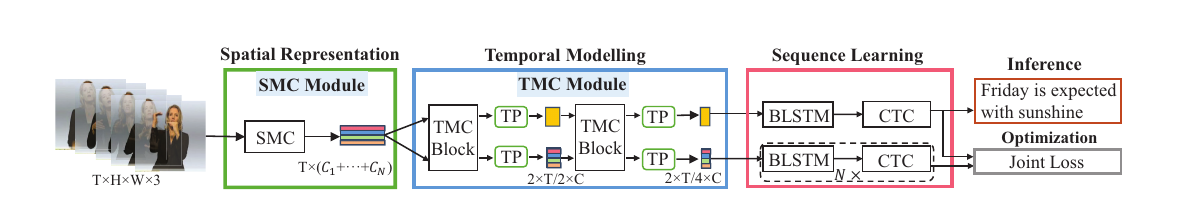
\includegraphics[width=\textwidth]{STMC/STMC.png}
    \caption{Estructura del modelo STMC}
\end{figure}

\subsubsection*{\underline{Spotter+GPT (Traducción Híbrida de SLT)}}
Aunque la traducción de la lengua de signos se ha formulado frecuentemente como una tarea de traducción automática neuronal compleja debido a los desafíos para alinear y tokenizar videos, además de las marcadas diferencias gramaticales entre lenguajes hablados y de signos, el enfoque propuesto por Sincan et al. \cite{} en \textsc{2024} innova al prescindir del entrenamiento de un modelo de traducción glosa-a-texto.
A diferencia de los enfoques convencionales que pueden presentar un bajo rendimiento en dominios extensos, el método \textbf{Spotter+GPT} propone una arquitectura híbrida que combina el reconocimiento visual clásico con las capacidades de razonamiento de un \textbf{LLM} preentrenado.
Para lograr esto, la arquitectura del sistema se divide en dos componentes principales:
\begin{itemize}
    \item \textbf{Módulo de Detección Visual (\textit{Sign Spotter})} que utiliza un modelo I3D entrenado con un gran conjunto de datos de dominio lingüístico para identificar signos individuales.
    Este módulo procesa el video continuo mediante una técnica de ventana deslizante para extraer predicciones de glosas, aplicando posteriormente un filtrado basado en umbrales de confianza para consolidar la secuencia.

    \item \textbf{Módulo de Generación de Lenguaje (\textit{ChatGPT / LLM})} que emplea la versión \textit{gpt-3.5-turbo} para recibir la secuencia de glosas detectadas de forma directa.
    Mediante ingeniería de instrucciones (\textit{prompting}) y sin requerir ajuste fino (\textit{fine-tuning}), el modelo transforma esta lista en una oración coherente en lenguaje hablado, superando de forma dinámica las diferencias en el orden gramatical.
\end{itemize}

\begin{figure}[H]
    \centering
    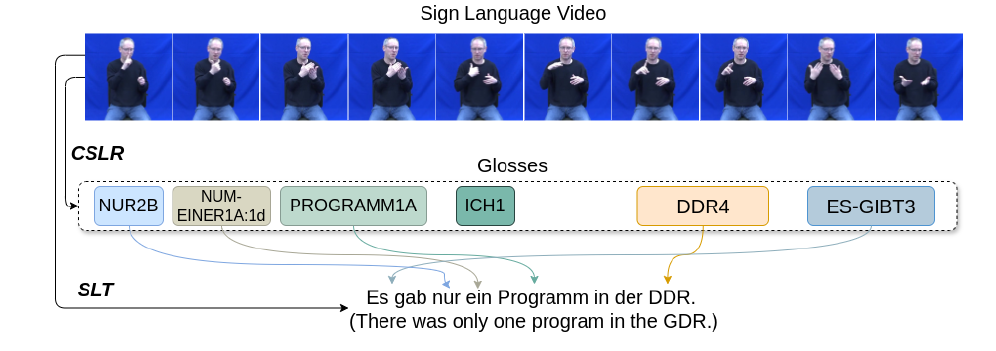
\includegraphics[width=\textwidth]{SPOTTER+GPT/SPOTTER.png}
    \caption{Estructura del modelo spotter+GPT}
\end{figure}

En cuanto a los resultados, los experimentos muestran que el Spotter+GPT supera a modelos secuenciales dedicados en métricas de calidad humana y similitud semántica (como BLEURT).
Además, destaca cualitativamente por su gran resiliencia, logrando mantener la coherencia semántica en la oración hablada final incluso cuando el detector visual pierde información o introduce glosas adicionales.


\begin{itemize}
    \item Transformers
\end{itemize}

\subsection{Modelos \textit{End2End}}
\begin{itemize}
    \item Gloss-Free SLT
    \item Sign2GPT (El Paradigma Gloss-based con LLM)
\end{itemize}

\subsection{LLMS para la traduccion de signos}

\section{Uso de keypoints como entrada a modelos en SL}

\section{Datasets}
El paradigma en cuanto conjuntos de datos no es muy diferente al de hace unos años.
Esto radica principalmente en la dificultad y el coste que existe en la traducción manual de miles de videos de legua de signos.
 % SOTA

\chapter{Fundamentos}

\section{Medidas de precisión en traducción}

\section{Transformers}
La aparición de la arquitectura \textbf{transformer}, introducida por \textit{Vaswani et al.} \cite{vaswani2023attentionneed}, supuso un cambio de paradigma en el procesamiento de secuencias, desplazando a las redes recurrentes en tareas de modelado de lenguaje. La relevancia de este modelo en el presente trabajo radica en su capacidad para gestionar dependencias de largo alcance mediante el mecanismo de auto-atención (\textit{self-attention}), el cual permite que cada elemento de una secuencia (ya sea una palabra o un \textit{keypoint} del cuerpo) sea procesado en relación con todos los demás de forma paralela. Por ello, dedicaremos esta sección a entender el funcionamiento de los \textit{transformers} con cierto nivel de detalle.

\subsection{¿Por qué Transformers?}
Para entender la relevancia e inovación de los transformers es necesario conocer lo que les precedía. En particular, las \textit{long short-term memory} y las \textit{gated recurrent neural networks} dominaron el procesamiento de secuencias mediante mecanismos de computación recurrente, los cuales procesan la información de manera secuencial siguiendo el orden temporal de la entrada. Estas arquitecturas presentaban dos limitaciones fundamentales: la dificultad para captar dependencias de largo alcance debido al desvanecimiento del gradiente y la imposibilidad de paralelizar el entrenamiento, lo que restringe enormemente la eficiencia computacional con secuencias largas.

Los transformers proponen abandonar por completo la recurrencia en favor del mecanismo de atención, lo que les permite captar dependencias de largo alcance en los textos de forma directa y con operaciones fácilmente paralelizables. En lugar de procesar la secuencia elemento a elemento, estos modelos consideran simultáneamente todos los tokens de entrada mediante el mecanismo de auto-atención, que calcula la relevancia relativa entre cada par de posiciones de la secuencia.

Este enfoque introduce varias ventajas clave. En primer lugar, elimina la dependencia estrictamente secuencial del cómputo, permitiendo un uso mucho más eficiente del hardware moderno, especialmente en arquitecturas paralelas como las \textbf{GPUs}. En segundo lugar, facilita el modelado de relaciones a larga distancia sin los problemas asociados al desvanecimiento del gradiente, ya que cualquier elemento de la secuencia puede interactuar directamente con cualquier otro en un solo paso de atención.

Además, los transformers incorporan mecanismos como las codificaciones posicionales para preservar la información sobre el orden de la secuencia, compensando así la ausencia de recurrencia. Esta combinación de atención global y representación posicional ha demostrado ser altamente efectiva en tareas de modelado del lenguaje y traducción automática, superando ampliamente a las arquitecturas recurrentes tradicionales.

Es natural plantearse si esta habilidad y facilidad que presentan los transoformers en la traducción de lenguajes se translada a la lengua de signos utilizando los \textit{keypoints} como representación de los signos.

\subsection{Codificación Posicional} % \textit{Positional Encoding}}

\subsection{Mecanismo de Auto-atención} % \textit{Self-Attention Mechanism}
La función de atención es un mecanismo que permite a un modelo identificar y priorizar la información más relevante dentro de un conjunto de datos. Para ello, compara una consulta, \textit{query} con un conjunto de claves, \textit{keys}, mediante una función de compatibilidad, que mide qué tan bien coincide la \textit{query} con cada \textit{key}, generando pesos que reflejan la importancia de cada elemento. Con base en estos pesos, se calcula una combinación ponderada de los valores \textit{values}, produciendo así una representación que enfatiza los componentes más pertinentes.

La función de atención más relevante es la \textit{Scaled Dot-Product Attention} cuya entrada son claves y consultas de dimensión $d_k$ y valores de dimensión $d_v$. En la práctica sacando provecho de que la multiplicación entre matrices está muy optimizada estas operaciones se hacen mediante matrices, obteniendo la siguiente fórmula.
\begin{equation*}
Attention(Q,K,V) = softmax\left( \frac{QK'}{\sqrt{d_k}}\right)V.
\end{equation*} Se añade el factor de escalado $\sqrt{d_k}$ pues si las matrices de \textit{query} y \textit{key} son de una muy alta dimensión, es posible que los valores exploten en tamaño donde la función \textit{softmax} se vuelve muy ``extrema'', es decir, asigna casi todo el peso a un solo elemento y hace que los gradientes sean muy pequeños, dificultando el entrenamiento.
\begin{figure}[H]
\center
\begin{tikzpicture}[
    % Estilo base
    block/.style={
        rectangle,
        draw=black,
        line width=1.5pt,
        rounded corners=2pt,
        minimum width=2.5cm,
        minimum height=0.8cm,
        font=\sffamily\Large,
        align=center
    },
    % Cambiamos 'scale' por 'styleScale' para evitar el error de pgfkeys
    styleMatmul/.style={block, fill=blue!15!purple!20},
    styleScale/.style={block, fill=yellow!25},
    styleMask/.style={block, fill=red!15},
    styleSoftmax/.style={block, fill=green!15},
    arrow/.style={-Stealth, line width=1.2pt}
]

    % --- NODOS ---
    \node (Q) at (0,0) {\sffamily\Large Q};
    \node (K) at (2,0) {\sffamily\Large K};
    \node (V) at (4,0) {\sffamily\Large V};

    % Columna central (usando el nuevo nombre de estilo styleScale)
    \node[styleMatmul, above=0.8cm of $(Q)!0.5!(K)$] (mm1) {MatMul};
    \node[styleScale, above=0.6cm of mm1] (sc) {\text{Scale}};
    \node[styleMask, above=0.6cm of sc] (mask) {Mask (opt.)};
    \node[styleSoftmax, above=0.6cm of mask] (sm) {SoftMax};

    % Bloque superior
    \node[styleMatmul, minimum width=4cm, above=0.8cm of sm, xshift=1.4cm] (mm2) {MatMul};

    % Salida
    \node (out) [above=0.7cm of mm2] {};

    % --- CONEXIONES ---
    \draw[arrow] (Q.north) -- ([xshift=-1cm]mm1.south);
    \draw[arrow] (K.north) -- ([xshift=1cm]mm1.south);
    \draw[arrow] (mm1) -- (sc);
    \draw[arrow] (sc) -- (mask);
    \draw[arrow] (mask) -- (sm);
    \draw[arrow] (sm.north) -- ([xshift=-1.4cm]mm2.south);
    \draw[arrow] (V.north) -- ([xshift=1.6cm]mm2.south);
    \draw[arrow] (mm2.north) -- (out);

\end{tikzpicture}
\caption{Una cabeza de atención}
\end{figure}







\shorthandoff{<}
\shorthandoff{>}
\begin{figure}[H]
\center
\begin{tikzpicture}[
    box/.style={
        rectangle,
        draw=black,
        line width=1.5pt,
        rounded corners=2pt,
        minimum width=2.5cm,
        minimum height=0.8cm,
        font=\sffamily\Large,
        align=center
    },
    smallbox/.style={
        rectangle,
        draw=black,
        line width=1.5pt,
        rounded corners=2pt,
        minimum width=1.8cm,
        minimum height=0.8cm,
        font=\sffamily\Large,
        align=center
    },
    arrow/.style={->, line width=1.2pt},
]

% Inputs
\node (V) at (-3,0) {V};
\node (K) at (0,0) {K};
\node (Q) at (3,0) {Q};


% === STACKED BACKGROUND (dibujar primero) ===
\foreach \i in {3,2,1} {
    \node[box, fill=purple!30,
        minimum width=8cm, minimum height=1.2cm, xshift=\i*6pt, yshift=\i*4pt, opacity=0.25] (att_box_\i) at (0,4) {};
    \node[smallbox, fill=gray!20,
          xshift=\i*3pt, yshift=\i*3pt, opacity=0.3] at (-3,1.5) {};
    \node[smallbox, fill=gray!20,
          xshift=\i*3pt, yshift=\i*3pt, opacity=0.3] at (0,1.5) {};
    \node[smallbox, fill=gray!20,
          xshift=\i*3pt, yshift=\i*3pt, opacity=0.3] at (3,1.5) {};
}

% === MAIN (dibujar al final, encima) ===
\node[box, fill=purple!30, minimum width=8cm] (attn) at (0,4)
{Scaled Dot-Product\\Attention};

% Linear layers
\node[smallbox, fill=gray!20] (linV) at (-3,1.5) {Linear};
\node[smallbox, fill=gray!20] (linK) at (0,1.5) {Linear};
\node[smallbox, fill=gray!20] (linQ) at (3,1.5) {Linear};

\node[box, fill=yellow!30] (concat) at (0,6) {Concat};
\node[box] (linear) at (0,7.5) {Linear};

% Arrows
\draw[arrow] (V) -- (linV);
\draw[arrow] (K) -- (linK);
\draw[arrow] (Q) -- (linQ);

\draw[arrow] (linV.north) -- ([xshift=-3cm]attn.south);
\draw[arrow] (linK.north) -- (attn.south);
\draw[arrow] (linQ.north) -- ([xshift=3cm]attn.south);

\draw[arrow] (attn) -- (concat);
\draw[arrow] (concat) -- (linear);

% h label
\node at (4.5,4) {$h$};

\end{tikzpicture}
\end{figure}
\shorthandon{<}
\shorthandon{>}

 % Fundamentos

\chapter{Metodología}
Modelos que vamos a probar, preprocesado de datos (normalización, etc)
\section{Extracción de Keypoints}
Como se mencionó, la extracción de keypoints es el proceso mediante el cual se obtiene una representación estructurada del cuerpo humano a partir de imágenes o vídeo, en forma de coordenadas de puntos anatómicos predefinidos, tales como articulaciones, extremidades o rasgos faciales. Esta representación abstrae la información visual relevante para el movimiento y la postura, descartando información irrelevante como el fondo, la iluminación o la apariencia superficial, lo que la convierte en una representación compacta, generalizable y respetuosa con la privacidad, tal y como se argumentó en la sección anterior.

En los últimos años, el avance conjunto de la visión por computador y el aprendizaje profundo ha dado lugar a herramientas de estimación de pose de gran precisión y eficiencia. Entre las más destacadas se encuentran \textbf{MediaPipe Holistic}, desarrollada por Google y ampliamente adoptada en la literatura de lengua de signos por su capacidad para detectar simultáneamente cuerpo, manos y rostro en tiempo real con un \textit{bajo costo en recursos computacionales}; \textbf{OpenPose}, uno de los primeros sistemas de estimación multi-persona de referencia, si bien \textit{ha sido ampliamente utilizado como referencia} en trabajos previos de estimación de pose, presenta limitaciones en términos de eficiencia y robustez frente a enfoques más recientes; aunque métodos como \textbf{HRNet} ofrecen una \textit{elevada precisión en la localización de keypoints en imágenes estáticas}, no incorporan de forma explícita mecanismos de seguimiento temporal, lo que puede generar variabilidad entre frames en secuencias de vídeo. Finalmente, \textbf{AlphaPose}, un sistema de estimación de pose de alta precisión que destaca especialmente en escenarios con múltiple personas, \textit{condiciones de oclusión y videos de baja calidad}, que es espeicalmete nuestro caso. Además, este último, a diferencia de \textbf{HRNet}, está optimizado para ser relativamente rápido, permitiendo una extracción más cómoda.




%\subsection{OpenPose}
\subsection{Alphapose}
AlphaPose ha demostrado obtener el menor error medio en detección de keypoints frente a MediaPipe y OpenPose incluso bajo condiciones de degradación de imagen \cite{info16110970}, lo que refuerza su idoneidad para entornos de grabación no controlados, habituales en datasets de lengua de signos, especialmente en el dataset con el que trabajaremos.

AlphaPose ofrece la capacidad de cambiar el modelo utilizado para la representación del esqueleto, existiendo principalmente dos conjuntos de datos de pose de cuerpo completo:
\begin{itemize}
  \item \textbf{COCO-WholeBody}, una ampliación del conjunto de datos \textbf{MS COCO} enfocada en el cuerpo humano completo. Incluye anotaciones detalladas de puntos clave del cuerpo, manos, cara y pies, lo que permite realizar estimaciones de pose más completas y precisas en tareas de análisis del movimiento humano.
  \item \textbf{HALPE-136}, un conjunto de datos más reciente que proporciona una anotación aún más densa (136 puntos clave), con especial énfasis en manos y rostro. Este mayor nivel de detalle puede resultar beneficioso en tareas que requieren capturar movimientos finos, como el reconocimiento de lengua de signos, aunque a costa de una mayor complejidad computacional y posible sensibilidad al ruido en entornos no controlados.
\end{itemize}
\begin{figure}[htbp]
  \centering
  % --- BLOQUE IZQUIERDO: La figura alta ---
  \begin{minipage}[b]{0.48\textwidth}
    \centering
    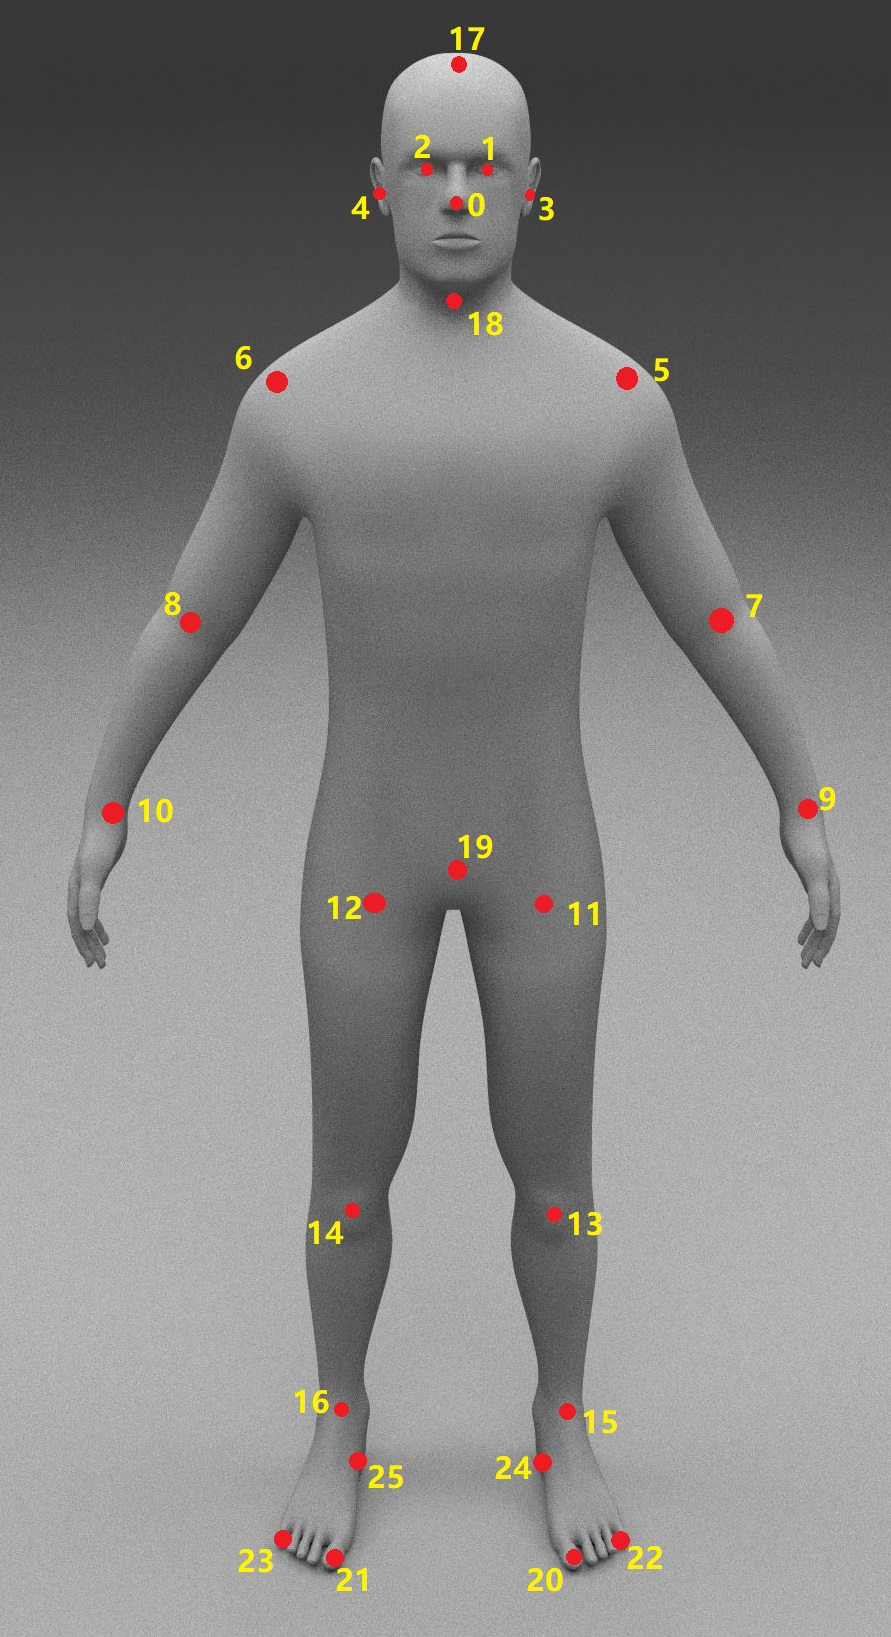
\includegraphics[width=\textwidth]{human_model_halpe_136.jpg}

  \end{minipage}
  \hfill
  % --- BLOQUE DERECHO: Las dos figuras cuadradas ---
  \begin{minipage}[b]{0.48\textwidth}
    \centering
    % Primera figura cuadrada
    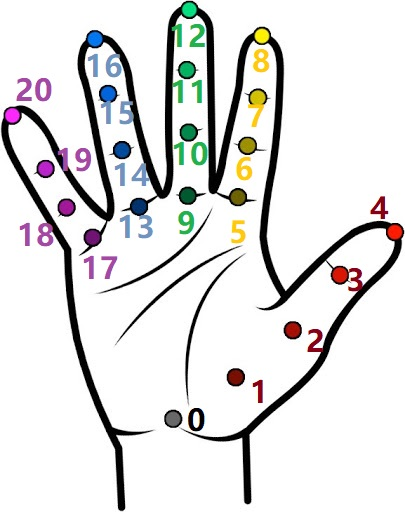
\includegraphics[width=0.8\textwidth]{hand_halpe_136.jpg}

    \vspace{0.5cm}

    % Segunda figura cuadrada
    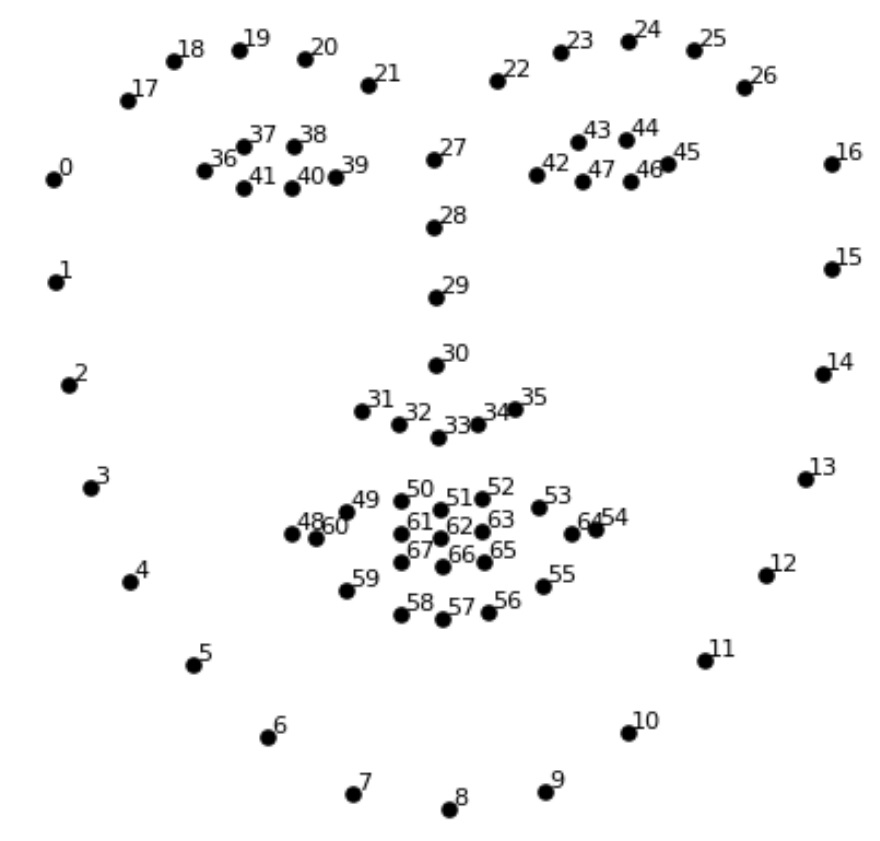
\includegraphics[width=0.8\textwidth]{face_halpe_136.jpg}

  \end{minipage}
  \caption{Keypoints en el Modelo Halpe-136}
\end{figure}

\lstinputlisting[language=json]{code/keypoints-format.txt}


\section{Seq2Seq}

\section{Normalización de los Datos}

\section{Multi Stream Keypoint Attention}
En esta sección se presentará la arquitectura principal del modelo \textit{Multi-stream Keypoint Attention} (MSKA) detallando el razonamiento detrás de la misma. Es importante notar que este modelo \textbf{no} es \textit{end-to-end}, hace uso de las glosas como representación intermedia de la traducción, asegurando que el modelo realmente aprende el significado detrás de los \textit{keypoints}.



 % Metodologia

\chapter{Experimentación y análisis de resultados}

\section{Ablation study}

\section{Comparativa con state of the art}

\section{También comparar la eficiencia}
 % Experimetancion

\chapter{Conclusión y trabajo futuro}\label{ch:conclusion}


Un dato revelador es que el WER sobre el conjunto de entrenamiento se sitúa en torno al $7\%$, frente al $27\%$ obtenido en dev y test.

Esta brecha de aproximadamente $20$ puntos porcentuales es una señal clara de sobreajuste: el modelo memoriza con alta precisión las secuencias de glosas del corpus de entrenamiento pero generaliza de forma limitada a muestras no vistas.

Este fenómeno es esperable dado el tamaño reducido del corpus ($7.096$ muestras de entrenamiento) y la complejidad de la arquitectura.

El hecho de que ninguna de las técnicas de aumentación logre cerrar significativamente esta brecha refuerza la hipótesis de que el problema no es trivialmente soluble mediante perturbaciones sobre los keypoints, y apunta a la necesidad de datos adicionales o estrategias de regularización más agresivas como líneas de trabajo futuro.
 % Conclusion

% Bibliografía
\begin{thebibliography}{99}

% ESTADO DEL ARTE
\bibitem{CamgozSLT} \textsc{Necati Cihan Camgoz, Oscar Koller, Simon Hadfield y Richard Bowden}, \textit{Sign Language Transformers: Joint End-to-end Sign Language Recognition and Translation}, arXiv preprint, art. 2003.13830, 2020. Disponible en: \url{https://arxiv.org/abs/2003.13830}

\bibitem{STMC_CSLR} \textsc{Hao Zhou, Wengang Zhou, Yun Zhou y Houqiang Li}, \textit{Spatial-Temporal Multi-Cue Network for Continuous Sign Language Recognition}, CoRR, vol. abs/2002.03187, 2020. Disponible en: \url{https://arxiv.org/abs/2002.03187}


\bibitem{GlossFreeSLT} \textsc{Benjia Zhou, Zhigang Chen, Albert Clapés, Jun Wan, Yanyan Liang, Sergio Escalera, Zhen Lei y Du Zhang}, \textit{Gloss-free Sign Language Translation: Improving from Visual-Language Pretraining}, arXiv preprint, art. 2307.14768, 2023. Disponible en: \url{https://arxiv.org/abs/2307.14768}

\bibitem{TwoStream-SLR} \textsc{Yutong Chen, Ronglai Zuo, Fangyun Wei, Yu Wu, Shujie Liu y Brian Mak}, \textit{Two-Stream Network for Sign Language Recognition and Translation}, arXiv preprint, art. 2211.01367, 2023. Disponible en: \url{https://arxiv.org/abs/2211.01367}

\bibitem{SignBERT} \textsc{Hezhen Hu, Weichao Zhao, Wengang Zhou y Houqiang Li}, \textit{SignBERT+: Hand-Model-Aware Self-Supervised Pre-Training for Sign Language Understanding}, IEEE Transactions on Pattern Analysis and Machine Intelligence, vol. 45, no. 9, pp. 11221-11239, 2023. Disponible en: \url{http://dx.doi.org/10.1109/TPAMI.2023.3269220}

\bibitem{info16110970} \textsc{Nada E. Elshami, Ahmad Salah, Amr Abdellatif y Heba Mohsen}, \textit{Toward Robust Human Pose Estimation Under Real-World Image Degradations and Restoration Scenarios}, Information, vol. 16, no. 11, art. 970, 2025. Disponible en: \url{https://www.mdpi.com/2078-2489/16/11/970}

\bibitem{alphapose} \textsc{Hao-Shu Fang, Jiefeng Li, Hongyang Tang, Chao Xu, Haoyi Zhu, Yuliang Xiu, Yong-Lu Li y Cewu Lu}, \textit{AlphaPose: Whole-Body Regional Multi-Person Pose Estimation and Tracking in Real-Time}, IEEE Transactions on Pattern Analysis and Machine Intelligence, 2022. Disponible en: \url{https://github.com/Fang-Haoshu/Halpe-FullBody}

\bibitem{mediapipe} \textsc{Camillo Lugaresi, Jiuqi Tang, Hadon Nash, Chris McClanahan, Eeshan Uboweja, Michael Hays et al.}, \textit{MediaPipe Holistic: Simultaneous Face, Hand and Pose Prediction, on device}, Google AI Blog, 2020.

\bibitem{OpenPose} \textsc{Z. Cao, G. Hidalgo Martinez, T. Simon, S. Wei y Y. A. Sheikh}, \textit{OpenPose: Realtime Multi-Person 2D Pose Estimation using Part Affinity Fields}, IEEE Transactions on Pattern Analysis and Machine Intelligence, 2019.

\bibitem{zhiliang2025deep} \textsc{L. Zhiliang y L. Zhuo}, \textit{Deep learning-based approaches for human pose estimation in interdisciplinary physics applications}, Scientific Reports, vol. 15, art. 42883, 2025. Disponible en: \url{https://doi.org/10.1038/s41598-025-26972-4}

\bibitem{vaswani2023attentionneed} \textsc{Ashish Vaswani, Noam Shazeer, Niki Parmar, Jakob Uszkoreit, Llion Jones, Aidan N. Gomez, Lukasz Kaiser e Illia Polosukhin}, \textit{Attention Is All You Need}, arXiv preprint, art. 1706.03762, 2023. Disponible en: \url{https://arxiv.org/abs/1706.03762}



\bibitem{fang2017rmpe} \textsc{Hao-Shu Fang, Shuqin Xie, Yu-Wing Tai y Cewu Lu}, \textit{RMPE: Regional Multi-person Pose Estimation}, Proceedings of the IEEE International Conference on Computer Vision (ICCV), 2017.

\bibitem{li2019crowdpose} \textsc{Jiefeng Li, Can Wang, Hao Zhu, Yihuan Mao, Hao-Shu Fang y Cewu Lu}, \textit{Crowdpose: Efficient crowded scenes pose estimation and a new benchmark}, Proceedings of the IEEE/CVF Conference on Computer Vision and Pattern Recognition (CVPR), pp. 10863-10872, 2019.

\bibitem{Phoenix} \textsc{Necati Cihan Camgoz, Simon Hadfield, Oscar Koller, Hermann Ney y Richard Bowden}, \textit{Neural Sign Language Translation}, 2018 IEEE/CVF Conference on Computer Vision and Pattern Recognition, pp. 7784-7793, 2018. Disponible en: \url{https://doi.org/10.1109/CVPR.2018.00812}


\bibitem{CSL-Daily} \textsc{Hao Zhou, Wengang Zhou, Weizhen Qi, Junfu Pu y Houqiang Li}, \textit{Improving Sign Language Translation with Monolingual Data by Sign Back-Translation}, IEEE/CVF International Conference on Computer Vision and Pattern Recognition (CVPR), 2021.

\bibitem{How2Sign} \textsc{Amanda Duarte, Shruti Palaskar, Lucas Ventura, Deepti Ghadiyaram, Kenneth DeHaan, Florian Metze, Jordi Torres y Xavier Giro-i-Nieto}, \textit{How2Sign: A Large-scale Multimodal Dataset for Continuous American Sign Language}, arXiv preprint, art. 2008.08143, 2021. Disponible en: \url{https://arxiv.org/abs/2008.08143}

\bibitem{sign4all} \textsc{F. Morillas-Espejo y E. Martínez-Martín}, \textit{Sign4all: a Spanish Sign Language dataset}, Scientific Data, vol. 13, no. 1, 2026. Disponible en: \url{https://doi.org/10.1038/s41597-026-06872-6}

\bibitem{docio2022eccv} \textsc{Laura Docío-Fernández et al.}, \textit{ECCV 2022 Sign Spotting Challenge: Dataset, Design and Results}, Proceedings of the European Conference on Computer Vision (ECCV) Workshops, Springer, 2022. Disponible en: \url{https://doi.org/10.1007/978-3-031-25085-9_13}

\bibitem{guo2025bridgingsignspokenlanguages} \textsc{Jianyuan Guo, Peike Li y Trevor Cohn}, \textit{Bridging Sign and Spoken Languages: Pseudo Gloss Generation for Sign Language Translation}, arXiv preprint, art. 2505.15438, 2025. Disponible en: \url{https://arxiv.org/abs/2505.15438}


\bibitem{MSKA} \textsc{Mo Guan, Yan Wang, Guangkun Ma, Jiarui Liu y Mingzu Sun}, \textit{Multi-Stream Keypoint Attention Network for Sign Language Recognition and Translation}, arXiv preprint, art. 2405.05672, 2024. Disponible en: \url{https://arxiv.org/abs/2405.05672}

\bibitem{SpotterGPT} \textsc{Ozge Mercanoglu Sincan y Richard Bowden}, \textit{Spotter+GPT: Turning Sign Spottings into Sentences with LLMs}, Adjunct Proceedings of the 25th ACM International Conference on Intelligent Virtual Agents, pp. 1-6, 2025. Disponible en: \url{http://dx.doi.org/10.1145/3742886.3756708}

\bibitem{SBleu} \textsc{Matt Post}, \textit{A Call for Clarity in Reporting BLEU Scores}, arXiv preprint, art. 1804.08771, 2018. Disponible en: \url{https://arxiv.org/abs/1804.08771}

\bibitem{paszke2019pytorch} \textsc{Adam Paszke, Sam Gross, Francisco Massa, Adam Lerer, James Bradbury, Gregory Chanan, Trevor Killeen, Zeming Lin, Natalia Gimelshein, Luca Antiga et al.}, \textit{PyTorch: An imperative style, high-performance deep learning library}, Advances in neural information processing systems, vol. 32, 2019.

\bibitem{wolf2020transformers} \textsc{Thomas Wolf, Lysandre Debut, Victor Sanh, Julien Chaumond, Clement Delangue, Anthony Moi, Pierric Cistac, Tim Rault, Sam Louf, Morgan Funtowicz et al.}, \textit{Transformers: State-of-the-art natural language processing}, arXiv preprint, art. 2010.11929, 2020.

\bibitem{huggingface2022evaluate} \textsc{Hugging Face}, \textit{Evaluate: A library for evaluating machine learning models}, 2022. Disponible en: \url{https://github.com/huggingface/evaluate}

\bibitem{DSTA} \textsc{Lei Shi, Yifan Zhang, Jian Cheng y Hanqing Lu}, \textit{Decoupled Spatial-Temporal Attention Network for Skeleton-Based Action Recognition}, arXiv preprint, art. 2007.03263, 2020. Disponible en: \url{https://arxiv.org/abs/2007.03263}

\bibitem{BLEU} \textsc{Kishore Papineni, Salim Roukos, Todd Ward y Wei-Jing Zhu}, \textit{Bleu: a Method for Automatic Evaluation of Machine Translation}, Proceedings of the 40th Annual Meeting of the Association for Computational Linguistics, pp. 311-318, 2002. Disponible en: \url{https://aclanthology.org/P02-1040/}

\bibitem{ROUGE} \textsc{Chin-Yew Lin}, \textit{ROUGE: A Package for Automatic Evaluation of Summaries}, Text Summarization Branches Out, pp. 74-81, 2004. Disponible en: \url{https://aclanthology.org/W04-1013/}

\bibitem{BLEURT} \textsc{Thibault Sellam, Dipanjan Das y Ankur P. Parikh}, \textit{BLEURT: Learning Robust Metrics for Text Generation}, arXiv preprint, art. 2004.04696, 2020. Disponible en: \url{https://arxiv.org/abs/2004.04696}

\bibitem{CTC} \textsc{Alex Graves, Santiago Fernández, Faustino Gomez y Jürgen Schmidhuber}, \textit{Connectionist temporal classification: Labelling unsegmented sequence data with recurrent neural networks}, ICML 2006 - Proceedings of the 23rd International Conference on Machine Learning, vol. 2006, pp. 369-376, 2006. Disponible en: \url{https://doi.org/10.1145/1143844.1143891}

\bibitem{JDrop} \textsc{Eirini Mathe, Ioannis Vernikos, Evaggelos Spyrou y Phivos Mylonas}, \textit{Leveraging Artificial Occluded Samples for Data Augmentation in Human Activity Recognition}, Sensors, vol. 25, no. 4, art. 1163, 2025. Disponible en: \url{https://www.mdpi.com/1424-8220/25/4/1163}

\bibitem{noise} \textsc{Chu Xin, Seokhwan Kim, Yongjoo Cho y Park Kyoung Shin}, \textit{Enhancing Human Action Recognition with 3D Skeleton Data: A Comprehensive Study of Deep Learning and Data Augmentation}, Electronics, vol. 13, no. 4, art. 747, 2024. Disponible en: \url{https://www.mdpi.com/2079-9292/13/4/747}

\bibitem{klDivergence} \textsc{Diako Rudd}, \textit{Understanding Kullback-Leibler (KL) Divergence}, Medium, 2024. Disponible en: \url{https://medium.com/@diako.rudd/understanding-kullback-leibler-kl-divergence-d77c976527c8}

\bibitem{mBART} \textsc{Yinhan Liu, Jiatao Gu, Naman Goyal, Xian Li, Sergey Edunov, Marjan Ghazvininejad, Mike Lewis y Luke Zettlemoyer}, \textit{Multilingual Denoising Pre-training for Neural Machine Translation}, CoRR, vol. abs/2001.08210, 2020. Disponible en: \url{https://arxiv.org/abs/2001.08210}

\bibitem{m2024machinetranslationlargelanguage} \textsc{Abhinav P. M., SujayKumar Reddy M y Oswald Christopher}, \textit{Machine Translation with Large Language Models: Decoder Only vs. Encoder-Decoder}, arXiv preprint, art. 2409.13747, 2024. Disponible en: \url{https://arxiv.org/abs/2409.13747}

\bibitem{qwen} \textsc{Qwen, An Yang, Baosong Yang, Beichen Zhang, Binyuan Hui, Bo Zheng, Bowen Yu, Chengyuan Li, Dayiheng Liu, Fei Huang, Haoran Wei, Huan Lin, Jian Yang, Jianhong Tu, Jianwei Zhang, Jianxin Yang, Jiaxi Yang, Jingren Zhou, Junyang Lin, Kai Dang, Keming Lu, Keqin Bao, Kexin Yang, Le Yu, Mei Li, Mingfeng Xue, Pei Zhang, Qin Zhu, Rui Men, Runji Lin, Tianhao Li, Tianyi Tang, Tingyu Xia, Xingzhang Ren, Xuancheng Ren, Yang Fan, Yang Su, Yichang Zhang, Yu Wan, Yuqiong Liu, Zeyu Cui, Zhenru Zhang y Zihan Qiu}, \textit{Qwen2.5 Technical Report}, arXiv preprint, art. 2412.15115, 2025. Disponible en: \url{https://arxiv.org/abs/2412.15115}

\bibitem{qwen2.5} \textsc{Qwen Team}, \textit{Qwen2.5: A Party of Foundation Models}, Qwen Blog, 2024. Disponible en: \url{https://qwenlm.github.io/blog/qwen2.5/}

\bibitem{LoRA} \textsc{Edward J. Hu, Yelong Shen, Phillip Wallis, Zeyuan Allen-Zhu, Yuanzhi Li, Shean Wang y Weizhu Chen}, \textit{LoRA: Low-Rank Adaptation of Large Language Models}, CoRR, vol. abs/2106.09685, 2021. Disponible en: \url{https://arxiv.org/abs/2106.09685}

\bibitem{LLaVA} \textsc{Haotian Liu, Chunyuan Li, Qingyang Wu y Yong Jae Lee}, \textit{Visual Instruction Tuning}, arXiv preprint, art. 2304.08485, 2023. Disponible en: \url{https://arxiv.org/abs/2304.08485}

\bibitem{llammlein} \textsc{Jan Pfister, Julia Wunderle y Andreas Hotho}, \textit{LLäMmlein: Transparent, Compact and Competitive German-Only Language Models from Scratch}, arXiv preprint, art. 2411.11171, 2025. Disponible en: \url{https://arxiv.org/abs/2411.11171}
\end{thebibliography}
 % Bib

\end{document}
